\chapter{Simple Applications}\label{ch:simpleapp}
%!TEX root = main.tex

In this chapter we explore a number of simple applications of the framework of probability on topics in religion.


\section{Atheism and Agnosticism}\label{sec:atheism_agnosticism}

Fewer words are as loaded and lead to as much disagreement on definitions as the terms {\em atheism} and {\em agnosticism} do.  In this work, we will define these words in a particular way, which we find the most consistent amongst the many different competing usages.  
\bi
\i Theism and atheism refer to {\em belief}
\i To be a {\em theist} simply means to believe in one, or more, personal gods.  This is in contrast to a {\em deist} who believes in an impersonal god.  Since deist beliefs are untestable,\TODO{explain why?} they are not addressed at all in this book.  Typically, we will be addressing the Christian or other monotheist arguments, but occasionally bring in polytheist beliefs as they apply.
\i To be an {\em atheist} simply means that one does not {\em believe} in the existence of any gods.  It is a statement of being unconvinced.  It is not a statement of confidence that there is no God, just that the arguments for the existence of God is unconvincing.
\i Gnosticism and agnosticism refers to {\em knowledge} (which is a subset of belief)
\i {\em Agnostics} believe that they cannot {\em know} whether there is a God or not, whole {\em gnostics} claim that {\em knowledge} can be had for (or against) the existence of God.  Thus, one can be an agnostic theist or agnostic atheist\footnote{Sometimes an agnostic atheist is called a weak-atheist, and a gnostic atheist a strong atheist, but we find these terms a bit too pejorative to use.}.  Also note, that {\em knowledge} is being used as described earlier, not as absolute certainty, but extremely high confidence. 
\ei

An analogy can help sort things out.  Say we have two explanations of the number of stars, one that
says there is an \emph{even} number of stars and another that says
 there is an \emph{odd} number of stars. Pretty much we know that,
at any given instant, one of these \emph{must} be true. However, strong
belief in either one is completely unwarranted - there is simply no way
to know. From a probabilistic framework, we express this as

\begin{eqnarray*}
P({\rm odd}) &=&0.5 \\\\
P({\rm even})&=&0.5
\end{eqnarray*}
Anyone making the strong claim that, for example, $P({\rm even})>0.95$ would have to present compelling evidence.  

\bi
\i Someone who is an {\em evenist} (analogous to a {\em theist}) would be someone convinced by the evidence, and assigns a high probability for $P({\rm even})$.  
\i Someone who is unconvinced by the evidence, say, an {\em a-evenist} (analogous to an {\em a-theist}) could maintain a lower probability for $P({\rm even})$.  
\i A {\em gnostic evenist} would have a very high probability for $P({\rm even})$, while an {\em agnostic evenist} would have a high, but not very high, probability for $P({\rm even})$.  
\i Likewise, a {\em gnostic a-evenist} would have a very low probability for $P({\rm even})$ (and thus a high $P({\rm odd})$), whereas an {\em agnostic a-evenist} would have a low $P({\rm even})$, and possibly equal to $P({\rm odd})$.  
\ei

Thus, for someone to be unconvinced of a claim (i.e. ``there are an even number of stars'') because they find the evidence unconvincing {\em does not} entail that they have a {\em belief} in the opposite (i.e. they do not necessarily believe there are an odd number of stars).  This point can't be made enough, because it is an extremely common misunderstanding, typically by Christians about atheists.

Matt Dillahunty clearly defines atheism as a lack of belief, and in a
court-room analogy says that he finds God ``not guilty of existing''. In
court, you find the plaintiff ``guilty'' or ``not guilty'', not
``guilty'' or ``innocent''. The burden of proof lies squarely with the
prosecution. If they haven't met that burden, then the jury finds the
plaintiff ``not guilty''. They may, or may not, believe that the
plaintiff is innocent. Establishing \emph{innocence} in the crime
changes the burden of proof to the defendant. The difference here comes
down to priors, which we can see through some illustrative examples
mapped to probability.

\subsection{Different Data}\label{different-data}

If we imagine data that might actually affect this prior probability,
the situation is a bit different. Let's imagine that through the laws of
physics we could demonstrate that

\begin{enumerate}
\def\labelenumi{\arabic{enumi}.}
\itemsep1pt\parskip0pt\parsep0pt
\item
  stars are nearly always formed in pairs
\item
  single stars are very short-lived
\end{enumerate}

we may actually have an argument for an even-number of stars in the
universe. In this case, we have \[
P(O|{\rm data}) \ll P(O)
\] and thus \[
P(E|{\rm data}) \gg P(E)
\]

Where one belief goes down, the other goes up. For our belief in
odd-ness to go down our belief in evenness must go up. We no longer
simply \emph{lack} a belief in odd-ness we also both \emph{believe} in
even-ness and \emph{believe} in non-odd-ness.

\subsection{More than two outcomes}\label{more-than-two-outcomes}

Something interesting happens when there are more than two outcomes.

\[
P(H)=P(R)=P(Y)=\frac{1}{3}
\]

Some data that nearly rules out one hypothesis, say \(R\), may not speak
to either other hypothesis directly, so you get the equal redistribution
like:

\begin{eqnarray}
\nonumber P(R)&\sim& 0 \\\\ 
\nonumber P(H)=P(Y)&\sim& 1/2 
\end{eqnarray}

or it might be the case that the data leaves unchanged the prior
probability of one of the hypotheses, raising the probability of the
other, like

\begin{eqnarray}
\nonumber P(R)&\sim& 0 \\\\ 
\nonumber P(H)&\sim& 1/3 \\\\
\nonumber P(Y)&\sim& 2/3 
\end{eqnarray}

Notice that it is possible to reduce the probability of one hypothesis
(i.e. \(R\)) and not effect the probability of a separate hypothesis
(i.e. \(H\)), when there are more than two outcomes. It is also possible
for the probability of that separate hypothesis (i.e. \(H\)) to go up,
or even go down. In other words, when there are more than one
hypothesis, presenting evidence for (or against) one hypothesis does not
always guarantee an adjustment in another hypothesis down (or up).





\section{Avoiding the Veneer of Objectivity}

There is a danger of using mathematics to give the
veneer of objectivity to an argument that is riddled with random
guesses, ill-defined concepts, and unsupported premises. In this section, we analyze some statements made in a podcast debate between theist Calum Miller and atheist James Crofta, expressed as probability statements\cite{Brierley:2014ab}.

\subsection{The Argument}\label{the-argument}

\ppquote{I think one useful way of thinking about is to consider
what evidence is in general. When we think about evidence for a theory,
in this case the theory is that God exists - we want to explain some
features of the world, we look for things (observations) which are
surprising if the theory isn't true but which aren't that surprising if
the theory is true.}{Calum Miller}

Calum Miller then goes on to do an analogy with fingerprints on a murder\TODO{include?}
weapon, as features of the world. He then points out the observation what he believes is evidence for God.

\ppquote{There are a number of arguments that work this way. But one of
the particular pieces of evidence that we want to discuss today is that
the world exhibits a real kind of regularity and there are basic laws,
science works, that we can understand the world. For all we know, the
universe could have been chaotic, might not have been any laws at all,
we might not have been able to do science - it might have been complete
chaos.}{Calum Miller}
\TODO{explain his quotes}

Here he's describing the form of the argument, as it might apply to the
sun rising.

\ppquote{Even more basic things that we use scientific reasoning for,
but do not always strike us as scientific truth. For example, \emph{`the
sun will rise tomorrow'}. Most of us believe that; this is a
common-sense inference from our observations. On atheism there is no reason to expect that regularity, because the sun could just fail to rise tomorrow.  On theism we can expect that kind of regularity because God set it in place}{Calum Miller}

Calum Miller finishes by describing further how moral responsibility hinges on this regularity, because we need to know the likely effect of my actions on others in order to make moral decisions and be responsible for them. If things were chaotic, if my actions had random effects, then moral responsibility could not work.

\subsection{The problem with the math - posteriors vs
likelihoods}\label{the-problem-with-the-math---posteriors-vs-likelihoods}

The first problem with Miller's argument, from a math point of view, is that he is simply comparing {\em part} of Bayes' rule (i.e the likelihoods, or how well the explanation fits the data) without looking at the rest of Bayes' rule (i.e. how likely, a-priori, those explanations are).  He compares the terms

\begin{eqnarray*}
\frac{P({\rm data}|{\rm theism})}{P({\rm data}|{\rm atheism})}
\end{eqnarray*}

and says that this is greater than one, and thus theism is more
likely. That is just the wrong question to ask. What we really want to
look at, even keeping the same structure, is the ratio of the
\emph{posterior} probabilities, or

\begin{eqnarray*}
\frac{P({\rm theism}|{\rm data})}{P({\rm atheism}|{\rm data})}
\end{eqnarray*}

which is related to the likelihood ratio through Bayes' rule:

\begin{eqnarray*}
\frac{P({\rm theism}|{\rm data})}{P({\rm atheism}|{\rm data})} &=& \frac{P({\rm data}|{\rm theism})}{P({\rm data}|{\rm atheism})} \times \frac{P({\rm theism})}{P({\rm atheism})}
\end{eqnarray*}
where we factor in the \emph{prior} probabilities. Already, we have an
issue, because the prior probability for the universe with an extra
agent should be smaller than one without such an agent\footnote{Recall this as a consequence of the Conjunction rule above.}. If you factor in
the agent with many specific properties, then this is smaller still.
By omitting this part, you could argue for anything. For example,

\begin{eqnarray*}
\frac{P({\rm data}|{\rm fairies})}{P({\rm data}|{\rm no-fairies})}>1
\end{eqnarray*}
or, in other words, the regularity of the universe is much more likely given fairies than no-fairies, so that is evidence for the fairies. Even if true, it is clearly an uninteresting and not a useful claim.

\subsection{The problem with the premise regarding
theism}\label{the-problem-with-the-premise-regarding-theism}

\TODO{this is good, need more like this}

The next problem is that it seems that Calum Miller is  trying
to sneak in many more details into his theism than his argument would
warrant. He needs to \emph{define} what he means by theism to state that
it is more likely to result in a regular universe. This is where the mathematics forces one to be specific and thorough, and thus highlights problems in arguments that may seem fine at their face.

For example, a number of counter examples can be made:

\begin{itemize}
\item  Under the Greek pantheon, it is more likely that things {\em would be chaotic}, at the will of capricious deities - thus $P({\rm data}|{\rm theism})$ would be lower than Calum Miller claims
\item  Gods or divine beings, such as Cthulhu, revel in chaos and thus would make it even less likely to result in a regular universe
\end{itemize}

So when Calum Miller says ``theism'', what he seems to mean is the existence of ``order-making God(s)'', but then his argument is circular: a regular universe is more likely under a regular-universe-making God hypothesis than not.

\subsection{The problem with the premise regarding
atheism}\label{the-problem-with-the-premise-regarding-atheism}

Further, Calum Miller never supports that it is unlikely to have an ordered universe under atheism. ``For all
we know, the universe could be chaotic'', Calum says. However, that
needs to be \emph{demonstrated}, not asserted, or it is an argument from
ignorance in disguise. It is possible, and in fact cosmology seems to be
pointing more in this direction, that the universe could not be any
other way - that the regularity is the result of the production of any
universe, and further that the production of universes is the only
stable solution. The notion of philosophical ``nothing'' may not be
physically realizable - it may be impossible for ``nothing'' to exist.\marginnote{Yes, I realize the verbal tangles one gets into with using the word ``nothing'' in the same sentence as ``exists''.  Unfortunately, I doubt English can do much better here.}


Calum Miller's introduction of morality to the argument adds nothing,
and only serves as a red herring. Without some regularity in the
universe, even thought itself would be impossible . We couldn't even
have the idea of a ``being'', or an animal, or life without regularity.
Thus, our mere existence requires regularity - but one that need not be
imposed from the outside, with a God. 

So, in summary, introducing the notion of a generic theism causes more problems to the argument than it solves, because it includes Zeus and Cthulhu. Circularity results when restricting the relevant theism to exclude these possibilities. Even if Calum Miller solved this, he is still answering the wrong question by ignoring the prior probabilities, and is at best achieving an uninteresting and useless result.


\section{Will the Sun rise tomorrow?}

Continuing with the Miller-Croft debate, Miller eventually brings up the analogy with evidence for the sun coming up as an example of knowledge claims and models.  The analogy fails when we look at the details of how this evidence is calculated.

Calum Miller describes philosopher David Hume on the justification for the sun rising tomorrow, and then continues with the analogy of model building in this situation,

\pquote{Hume basically noted that we don't have any non-circular
justification for thinking that the universe will be regular, that it
will continue to be regular in the future. {[}\ldots{}{]} He doesn't
just say that we have to be a bit unsure that the sun will rise
tomorrow, he says that we have no good reason at all for thinking the
sun will rise tomorrow. The most common justification that the sun will
rise tomorrow is that it has risen every day in the past. But then if
you compare two theories, one says that the sun rises everyday in the
past and in the future and the other theory says that the sun rises
everyday in the past but won't rise tomorrow. Both those theories
predict the observations we already have, both those theories lead us to
expect the observations, and so the observations we currently have don't
distinguish between these two theories. And yet one of those theories
predicts the sun will rise tomorrow and one of them predicts that the
sun won't rise tomorrow. So, even though we have those observations,
they don't really do an obviously good job of determining which of these
theories is true. {[}\ldots{}{]} He is saying that the past observations
don't give us that good reason for thinking that the sun will rise
tomorrow. This is the Problem of Induction and has perplexed
philosophers for centuries.}

\subsection{What does Hume say?}

It is instructive to note that Hume predates the mathematics of probability, and see what Hume {\em actually} says about the Sun rising\cite{Hume:1748aa},
\pquote{
Matters of fact, which are the second objects of human reason, are not
ascertained in the same manner; nor is our evidence of their truth,
however great, of a like nature with the foregoing. The contrary of
every matter of fact is still possible, because it can never imply a
contradiction, and is conceived by the mind with the same facility and
distinctness, as if ever so conformable to reality. That the sun will
not rise tomorrow is no less intelligible a proposition, and implies no
more contradiction, than the affirmation, that it will rise. We should
in vain, therefore, attempt to demonstrate its falsehood. Were it
demonstratively false, it would imply a contradiction, and could never
be distinctly conceived by the mind.}

Here Hume is essentially stating that all propositions have a non-zero
probability (however small they might be) unless they are
\emph{logically} impossible. This is not saying, at all, that we have no
good reason to believe the sun will rise tomorrow.


\pquote{The bread, which I formerly ate, nourished me: that is, a body of such
sensible qualities was, at that time, endued with such secret powers;
but does it follow, that other bread must also nourish me at another
time, and that like sensible qualities must always be attended with like
secret powers? The consequence seems nowise necessary.\cite{Hume:1748aa}
}

Again, although Hume predates probability theory, this is essentially
what he is saying - the consequence is not logically \emph{necessary}
(i.e. \(P({\rm consequence}|{\rm observations})<1\)). We see this as a
direct application of probability theory, a totally uncontroversial
application at that.

The so-called ``problem of induction'' to which Calum Miller refers is not really a problem. It is a direct consequence of the mathematics of probability, and thus is the result of mathematical axioms.  Hume is not claiming that there is {\em no} good reason to see the
consequence following from the the observations, only that he is unable to find a good reason,

\pquote{
The connection between these propositions is not intuitive. There is
required a medium, which may enable the mind to draw such an inference,
if indeed it be drawn by reasoning and argument. What that medium is, I
must confess, passes my comprehension, and it is incumbent on those to
produce it, who assert that it really exists, and is the origin of all
our conclusions concerning matter of fact.
}

The medium Hume refers to is simply the mathematics of probability,
something which post-dates Hume's writings. Hume was being honest that
he didn't see a way, and he did not claim that there was {\em no possible} way - that would be an ``argument from ignorance'' fallacy.

\subsection{What does Laplace say?}

Once we have probability theory, then we can actually do some simple
calculations concerning the probability of the sun rising tomorrow. Of
course these calculations are not a complete description of the problem,
but give the flavor of it. Laplace used the sunrise problem as an
example application of his Rule of Succession, which itself is derived
from the rules of probability. The calculation goes something like this.

\begin{itemize}
\itemsep1pt\parskip0pt\parsep0pt
\item
  Our model is that the sun rises with unknown probability \(p\)
\item
  Given complete ignorance of \(p\) we assume an initial uniform
  probability (all values are equivalent)
\item
  The sun has risen every day for the written record, say, 10000 years
\item
  the probability for rising tomorrow, which is also the mean value of
  \(p\) over the posterior probability, is given by the Rule of
  Succession\cite{Wikipedia:2015ab} (also known as the ``assume one success and one
  failure''\cite{Blais:2014aa}):
\end{itemize}

\newcommand{\yr}{\mbox{year}}
\renewcommand{\day}{\mbox{day}}
\beqn
P\left(\parbox{.7in}{rise\\tomorrow}\middle|\parbox{1in}{rose today,\\rose yesterday, \\$\ldots$,\\ on day 0}\right)&=&
\frac{10000 \yr \times 365 \day/\yr+1}{10000 \yr \times 365 \day/\yr+2}\\
&=&0.9999997
\eeqn

It gets
messier when you can't even assume that both a failure and a success
are possible, but it can
still be done without any change to the qualitative result.

Clearly we have quite good reasons to believe the that sun will rise
tomorrow.

\subsection{Two theories}\label{two-theories}

We go back to Calum Miller's two theories:

\pquote{
If you compare two theories, one says that the sun rises everyday in the
past and in the future and the other theory says that the sun rises
everyday in the past but won't rise tomorrow. Both those theories
predict the observations we already have, both those theories lead us to
expect the observations, and so the observations we currently have don't
distinguish between these two theories.
}

The situation for arguing a high probability of tomorrow's sun rise is
far more compelling, however, because our information is not simply that
the sun has risen in the past, but includes observations of the patterns
of the seasons, the predictions of the phases of the moon and Venus, and
a whole host of other factors which significantly increase the chance
the sun will rise. Laplace knew this well, and was using this example
not as a serious calculation, but as a pedagogical example.

As a consequence, both of Calum Miller's so-called theories do \emph{not}
predict the observations we already have - only one of them does. Even
if we accept just the observations for which both theories are
consistent in the past, one has to view this two-theory perspective from
the point of prediction. Imagine it's now tomorrow, and ``Theory B'' doesn't work - so we modify it to say the sun won't rise \emph{tomorrow} (the new tomorrow). That next day comes with a sunrise, and this ``Theory B 2.0'' is wrong (again) and has to be modified (again). It is clear that ``Theory B'' fails, and we should be less confident in it. That's why, in science, it isn't nearly enough to be consistent with past data - one must make predictions, not just post-dictions, and test it. It is often trivial to come up with ``explanations'' for data we already have - especially when we can be infinitely plastic in the models we propose. 



\section{Belief, Knowledge, and Scientific Literacy}

Concepts about belief and knowledge arose in the National Science Foundation survey on scientific literacy.  The NSF had decided to change the wording of two questions in the
survey. The original wording is 
\pquote{Human beings, as we know them today,
developed from earlier species of animals,} and \pquote{The universe began
with a huge explosion.}

 The new wording is \pquote{\underline{According to
evolutionary theory,} human beings, as we know them today, developed
from earlier species of animals''  (emphasis mine)} and 
\pquote{\underline{According to astronomers,}
the universe began with a huge explosion.'' (emphasis mine)}

 It is noted that there will be a transition period with the questions, with half of the surveys containing the new questions and half the old, to determine its effect.

The stated goal for this change, from the NSF, is to separate knowledge
from belief. You might \emph{believe} that humans are created in their
present form, 6000 years ago, but the new questions try to ascertain
whether you know that ``evolutionary theory'' says something different.
Is this an important distinction? Is this what we really want to
measure? Which is more important for a society? What is the difference
between knowledge and belief in this context?\marginnote{It is quite clear that there will be at least one effect for this
rewording: given that the US falls way behind other countries on science
literacy, especially with these particular questions, the rewording will
most likely increase these numbers with no other work done.}

Since beliefs are representations of the world that we hold to be correct for the real world\ldots{}as
opposed to hopes, which are also representations of the world but not
ones that we hold to be necessarily correct. Knowledge is, as we have defined, simply that collection
of beliefs that we hold with such high probability or, in other words,
with such confidence that we do not significantly doubt them. The belief
that the sun rises in the east each morning is considered knowledge for
the reason that we hold it with an extremely high probability. 

The NSF defines scientific literacy as
\href{http://www.nsf.gov/statistics/seind04/c7/c7s2.htm}{``knowing basic
facts and concepts about science and having an understanding of how
science works.''} Why is literacy important? Again,
\href{http://www.nsf.gov/statistics/seind04/c7/c7s2.htm}{the NSF}: ``It [literacy] is valuable not only in keeping up with important science-related issues, but also in evaluating and assessing the validity of any type of information and participating meaningfully in the political process.''

The question we must then ask is, does the new wording measure scientific literacy better than the old wording? To do this, we need to outline the four possible types of people answering the two forms of the questions:

\begin{enumerate}
\def\labelenumi{\arabic{enumi}.}
\itemsep1pt\parskip0pt\parsep0pt
\item
  people who answer ``yes'' to the old and ``yes'' to the new
\item
  people who answer ``no'' to the old and ``no'' to the new
\item
  people who answer ``no'' to the old and ``yes'' to the new
\item
  people who answer ``yes'' to the old and ``no'' to the new
\end{enumerate}

The wording change doesn't change cases 1 and 2, adds case 3 to the
``yes'' category and it introduces the erroneous case 4. The cases can
be summarized in another way, like

\begin{enumerate}
\def\labelenumi{\arabic{enumi}.}
\itemsep1pt\parskip0pt\parsep0pt
\item
  people who know both that, say, the universe began with a big
  explosion and that astronomers claim that this is true. This is
  indicative of scientific literacy.
\item
  people who don't know, or do not believe, that the universe began with
  a big explosion and that also don't know that astronomers claim that this
  is true. This is indicative of scientific \emph{illiteracy}.
\item
  people who don't \emph{believe} that the universe began with a big
  explosion but know that astronomers claim that this is true. (more on
  this below)
\item
  people who know that the universe began with a big explosion, but do
  not believe that astronomers claim that this is true. This might at
  first seem to be a totally unreasonable and marginal case, but we think
  it is more significant than perhaps is generally appreciated. These
  people might think that the new wording is a trick question (e.g.~they
  might think, for example, that \emph{physicists}, as opposed to astronomers, claim
  that it is true). I've had students answer questions in this way, so
  it is not quite as uncommon as one might think. These students
  overthink the problem: they know the fact, but are distracted by the
  extra complexity of the question, thinking that the test is trying to
  trick them.
\end{enumerate}

The only reason these particular questions were modified was because of
the prevalence of religious belief. How do we know this? We don't see a
proposal to change ``The Earth orbits around the Sun and takes a year to
do it'' to ``According to astronomers, the Earth orbits around the Sun
and takes a year to do it.'' Why? Because no religion (now) has a stake
in the answer to that question, and thus have no objection to the claim.
Of course, if you go back to the days of Copernicus this was a different
story and people were severely punished for too strongly making such a
claim. The two questions that are proposed to be changed in this way are
precisely the two concepts that crop up in every creationist tract, and
are clearly the two major stumbling blocks for a literalist reading of
the Bible or the Quran.

{\textbf{Case 3: The Religious Believer}}

Aside from the motivation for the change, we can ask the question
whether it is accomplishing something important anyway. Are these Case 3
people, who would answer ``no'' to the old question but ``yes'' to the
new question, demonstrating scientific literacy?  No.  What they've confirmed is that they know that some scientists \emph{claim}
that the universe began with an explosion, but they don't believe it.
This means that they don't accept either the data, or the methods, or both. If
the question were about something on the fringes of science, then
perhaps this is fine, but it isn't the case with these two questions.
Evolution theory, for example, is as well established as the Round Earth
theory and the Germ theory of disease. To deny it is to deny all of the
\emph{independent} work in molecular biology, embryology, ecology,
etc\ldots{} that supports it. Even though they may know the fact that
biologists support Evolution theory, they have not demonstrated any
scientific literacy in terms of ``evaluating and assessing the validity
of any type of information and participating meaningfully in the
political process.'' The same can be said of the Big Bang theory, to a
slightly lesser degree (i.e.~there isn't \emph{quite} the volume of
completely independent \emph{fields} of study supporting it, as there is
for Evolution, but the data is nearly incontrovertible anyway). To deny
either idea is akin to denying the Germ theory of disease.

Imagine someone answering ``no'' to the question ``The world is round''
but answers ``yes'' to ``According to geographers, the world is round''.
Would they be demonstrating scientific literacy?  The difference between belief, knowledge, and the claims of others is quite apparent in this application.


\section{Communicating Science}

Joan Roughgarden in
\href{http://thesciencenetwork.org/programs/beyond-belief-science-religion-reason-and-survival}{Beyond
Belief} made a very astute observation of a problem, and then proposed a
lousy solution to it. The problem she was addressing had to do with the
public perception of evolution as something quite uncertain
scientifically (``theory vs fact''). She observed that the public sees
science changing its stance on many things, especially in medicine. One
day, you should eat bran. The next, bran is bad for you. The next, bran
is good for you again. As a result, the public observes that \emph{some}
sciences are uncertain, and can't distinguish one field from another or
one type of claim from another, so they apply doubt to \emph{all} of
science even when it is not warranted by the science. Her solution
involves using religious analogies, interpreting phrases in the Bible to
explain things like natural selection and mutations, in order to
communicate it to a group of people who share and value that vocabulary.
Dawkins rightly chews her out for this approach, pointing out how far
she is stretching the meaning of the phrases just to fit her philosophy.

The problem she is stating, however, is quite real. How can we expect
the public to make decisions about medicine, global warming, evolution,
the big bang, etc\ldots{} when they (somewhat rightly, somewhat wrongly)
observe that the scientists themselves are arguing about it? The
Intelligent Design proponents are currently using this observation to sow
doubt with the public in their efforts to ``teach the controversy'' of
evolution to inject creationism into the schools. It is a failure of the
scientists, and the media that covers them, to communicate with the
public. Can we do better?

Here is a proposal, which we'll sketch out in a simplistic, yet illustrative, example. The problem
is not the communication of facts, or even of the procedures of science.
The problem is with the communication of \emph{uncertainties} - and thus the probabilities - associated with measurement. In day-to-day life, we easily handle claims with different levels of
uncertainties. The sun rises in the east each morning has low
uncertainty. The claims of the auto salesman or the politician have
higher uncertainty. Quantifying it is, of course, more challenging but
the qualitative features of uncertainty are known to nearly everyone. So
scientists and journalists really need to take efforts to communicate
the uncertainty of every claim, not just the fact of the claim or how
the new observations differ from the old observations. How could this be
done?  We think, at least roughly, one should include a plot of the
probability distribution with any claim. This distribution is a graphical representation of the weights of one's beliefs over all of the possible values of the measured quantity.  One doesn't need to know
advanced math to see the picture. If every claim is accompanied by a
plot of the uncertainties, the public will get used to reading them. Let
us demonstrate with a toy example.

Say, we are trying to determine the origin year of {\em homo sapiens}. We realize there isn't just one year, and there is a process, but it is not much harder to include those in this simple analysis.  We have several {\em homo sapiens} fossils where we've measured the age, allowing us to
calculate our best guess of the age, and the distribution of our
uncertainty shown here.

\begin{figure}[htbp]
\centering
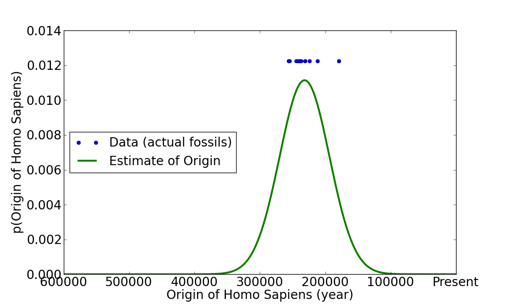
\includegraphics{img/blah2-2011-01-29-11-35.png}
\caption{Hypothetical distribution of ages for {\em homo sapiens}.}
\end{figure}

The details of this are unimportant, because the picture is pretty clear regardless of the details.  A few observations are in order here:

\begin{enumerate}
\def\labelenumi{\arabic{enumi}.}
\itemsep1pt\parskip0pt\parsep0pt
\item
  Our ``best guess'' is around the middle of this distribution, but it
  really can't be interpreted as ``homo sapiens originated 250,000 years
  ago'' as it might read in a newspaper
\item
  there are many possible values for the origin time of {\em homo sapiens} that lie well outside of our data yet have non-zero probability.  This means that these values could very well be the truth, and we are being up front about it.
\end{enumerate}

Now, we have a new paper that adds another fossil much older than than
the previous ones, around 340000 years ago. Currently, newspapers often make claims like ``origin of homo sapiens 150\% older than originally thought'', or ``estimates of the origin of humans overthrown by new data''. How might it look with the uncertainties plotted?

\begin{figure}[htbp]
\centering
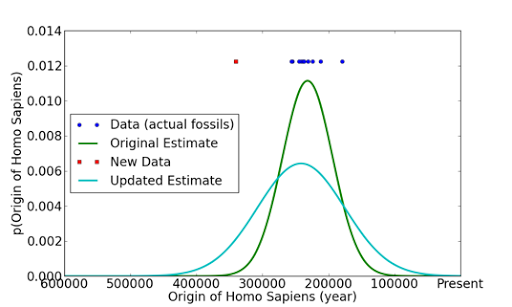
\includegraphics{img/blah3-2011-01-29-11-35.png}
\caption{Hypothetical distribution of ages for {\em homo sapiens}, with one added data point.}
\end{figure}

There are a number of lessons that can be read from this.

\begin{enumerate}
\def\labelenumi{\arabic{enumi}.}
\itemsep1pt\parskip0pt\parsep0pt
\item
  the new data updates our ``best estimate'' by only a little - the old
  data, combined with the new data, are used for the estimate
\item
  our uncertainties have widened - by having a larger range of data, our
  uncertainties may have increased with new data.
\end{enumerate}

In reality, estimating an origin (first event) will update a bit
differently than this example shows. For example, the uncertainties in
the right-half of the distribution may not be affected at all by an
older observation. If this data were in medicine, however, and we were
estimating the effect of some new treatment, then the update would be
very similar. A single result of a strong effect may not increase our
best estimate for that effect by a huge amount. The uncertainties in
many medical treatments, or dietary recommendations, straddle the
origin: there is significant probability for \emph{no effect}. It would
be fruitful to see the plot of uncertainties, pushed a little this way
and that, updated in perhaps a wiki style by scientists as new data come
in. There would be many lessons, all of which would help the public
understanding of science.

\begin{enumerate}
\def\labelenumi{\arabic{enumi}.}
\itemsep1pt\parskip0pt\parsep0pt
\item
  observations rarely overturn well-supported scientific understanding
\item
  not all topics have equal uncertainties - doubting everything the same
  amount is not rational
\item
  certainty is never an option, but sometimes the uncertainty is so low
  that there is a practical certainty
\item
  nature itself, not authority, determines our best guess and some of
  our uncertainty
\item
  if the thing you are measuring has a small effect, then you should
  expect a series of measurements of the effect to change sign: bran is
  good, bran is bad, bran is good, etc\ldots{}. This doesn't mean that
  the scientists are waffling, it only means that the effect is small
  and difficult to detect - and probably meaningless.
\end{enumerate}

I think the public could learn to, at least qualitatively, understand
and use plots like these. Perhaps there is a better way to display it
that does not do violence to the truth, and we'd be open to that.  We think getting in the habit of making plots like this would be good for the
scientist as well, forcing them to address and communicate the actual
uncertainties in their claims.  When we explore specific religions topic like miracles, this sort of thinking and communication of data could be critical.
